\section{Virtual Machines}

A \textbf{virtual machine monitor} (VMM) virtualizes an entire system. The execution environment of the VMs we’ll look at provide a simulation of the raw machine hardware.\medskip

While a VMM is the functionality required to create the illusions of real hardware, the \textbf{hypervisor} is the software that runs on real, physical hardware and supports multiple VMs (each with its associated virtual machine monitor). There is one hypervisor on which many VMMs can run. We call a hypervisor running on bare metal a type-1 (native) hypervisor and one running on a real OS a type-2 (hosted) hypervisor. \medskip

OS-level virtualization uses a single OS to provide the illusion of multiple \textbf{containers} of that OS. Code running in a container have the same system call interface as the underlying OS, but cannot access any device. This is achieved by limiting the file system namespace (by changing the root for each container) and the process namespace, so processes can only see processes which share their container. In general, using containers is more efficient than using hypervisors.


\subsection{The Uses of Virtual Machines}

When multiple applications contend for resources the performance of one or more may degrade in ways outside the control of the OS. \textbf{Resource isolation} guarantees to one application that its performance will not be impacted by others, this is done by running the application in a VM. \medskip

\textbf{Cloud computing} is the business of renting computing resources as a utility to paying customers rather than selling hardware. They are primarily based on renting computing resources in the form of a VM (similar to resource isolation).

The term \textbf{server consolidation} refers to taking a set of services, each running on a dedicated server, and consolidating them onto a single physical machine so that each runs in a VM. \medskip

\textbf{Backward compatibility} is the ability of a new machine to run programs (including OSes) written for an old machine. \medskip


\subsection{Virtualizing the CPU}

To run an OS inside a VM, we need to completely virtualize the processor, including the kernel (else we simply could use threads). The processor in the VM clearly cannot execute a privileged instruction "for real". Instead, the default result is a trap/fault: \medskip

\textit{Trap-and-emulate} is a technique for virtualization which runs privileged code in non-privileged mode. Any privileged instruction causes a trap to the VMM, which then emulates the instruction and returns to the VM guest code.\medskip

The problem is that there might be some instructions which do not cause a trap when run in non-privileged mode but have a different behavior when executed in kernel mode (e.g. \textit{POPF} in x86). This cannot happen with a strictly virtualizable ISA. \medskip

An ISA is \textbf{strictly virtualizable} iff it can be perfectly emulated over itself with all non-privileged instructions executed naively and all privileged instructions emulated via traps. \medskip

There are different approaches to dealing with non strictly virtualizable ISA:
\begin{itemize}
	\item \textbf{Full software emulation}: Creates a virtual machine by interpreting all kernel-mode code in software. This is very slow, especially for many I/O operations.
	\item \textbf{Paravirtualization}: A paravirtualized guest OS is one which has been specifically modified to run inside a VM. Critical calls are replaced with explicit trap instructions.
	\item \textbf{Binary rewriting}: Scans compiled kernel code for unvirtualizable instructions and rewrites them – essentially patching the kernel on the fly. This is done on demand: All kernel pages are first protected and when first accessed (i.e., the pro- tection trap occurs), they get scanned and rewritten.	
	\item \textbf{Virtualization extensions}: Convert ISA by adding virtualization extensions. This typically takes the form of a new processor mode. Today, both ARM and x86 do have hardware support for virtualization.
\end{itemize}


\subsection{Viratualizing the MMU}

With virutalization, there is a second level of indirection with memory addresses. Now, a physical memory address is not unique in the machine, but in one VM (guest OS thinks it is physical). Thus, we define the \textbf{machine address} to be a real address on the machine which gets translated from the guest OSs physical address. From the view of the hypervisor, the machine address is the physical address.

\begin{center}
	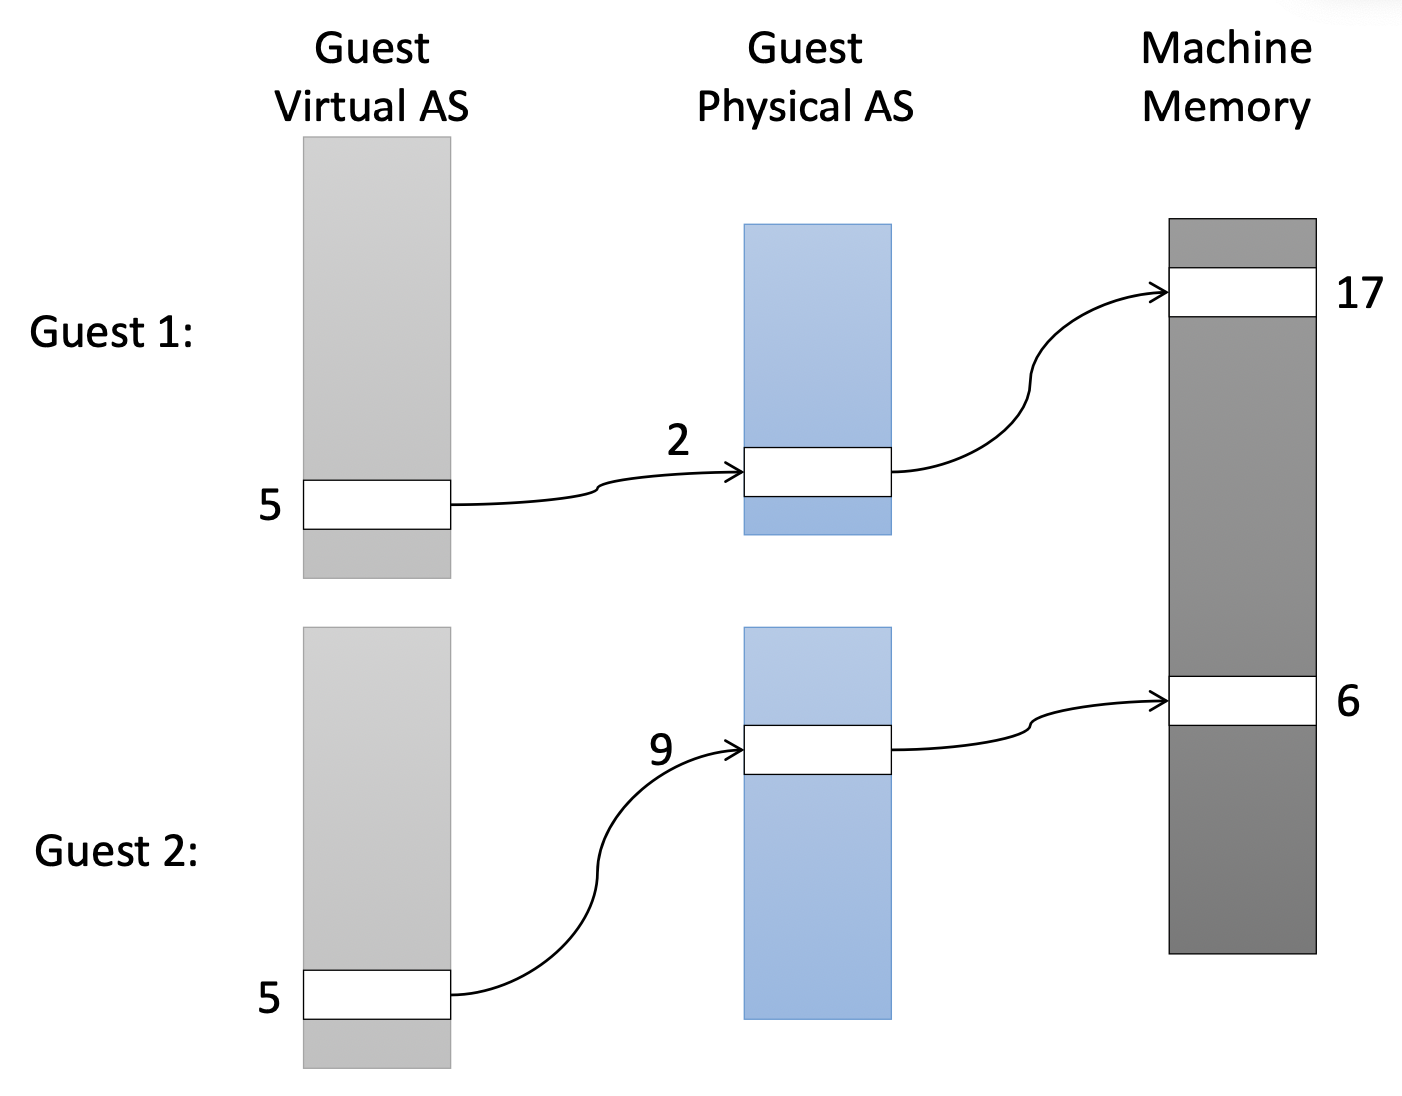
\includegraphics[width=0.7\linewidth]{virtual_mmu.png}
\end{center}

The hypervisor thus needs to translate a guest virtual address not to a guest physical address but to a machine address instead. There are several ways to do so:
\begin{itemize}
	\item Directly writable tables: The guest OS creates the page tables that the hardware uses to directly translate guest virtual to machine addresses. This requires paravirtualization. The VMM needs to check all writes to any PTE in the system. To change a PTBR, a hypercall is needed.
	\item A shadow page table is a page table maintained by the hypervisor which contains the result of translating virtual addresses through the guest OS’s page tables, and then the VMM’s physical-to-machine page table. The guest OS thus sets up its own PT, but they get never used. The VMM maintains the shadow PT which maps directly from guest VAs to machine addresses. \medskip
		
		The VMM must keep the shadow table consistent with both the guest’s PT and the hypervisors own physical-to-machine table. It achieves this by write-protecting all the guest OS's PT and trapping writes on them. When a write happens, it applies the update to the shadow page as well.
	\item Nested Paging/$2^{nd}$ level page translation is an enhancement to the MMU hardware that allows it to translate through two page tables (guest virtual to guest physical and guest physical to machine), caching the result (virtual to machine) in the TLB. This can be fast, but a TLB miss is costly.
\end{itemize}


\subsection{Viratualizing the Physical Memory}

How can the hypervisor allocate memory to a guest OS? The guest OS expects a fixed area of physical memory which does not change dynamically. In theory, this problem can be solved with paging. However, there is a phenomenon called \textbf{double paging}. Consider the following sequence of events:
\begin{enumerate}
	\item The hypervisor pages out a guest page $P$ to storage
	\item A guest OS decides to page out the virtual page associated with $P$ and touches it.
	\item This triggers a page fault in the hypervisor, hence $P$ gets paged back in memory.
	\item The page is immediately written out to disk and discarded by the guest OS.
\end{enumerate}
So to throw away a page in a guest OS, there are three I/O operations and one extra page fault! We could solve this problem with paravirtualization, but this introduces more complexity. \medskip

\textbf{Memory ballooning} is an elegant solution to this problem. It allows hypervisors to reallocate machine memory between VMs without incurring the overhead of double paging. A  device driver, the balloon driver, is installed in the guest kernel. This driver is VM-aware, i.e. it can make hypercalls and receive messages from the VMM. The principle is to block a large area of physical memory in the guest OS, which then can be allocated to the OS by unblocking it. \medskip

Memory can also be reclaimed from a guest OS (inflating the balloon):
\begin{enumerate}
	\item The VMM asks the balloon driver to return $n$ physical pages from the guest OS to the hypervisor.
	\item The balloon driver notifies the OS to allocate $n$ pages of memory for its private use.
	\item It communicates the guest-physical addresses of these frames to the VMM using a hypercall.
	\item The VMM unmaps these pages from the guest OS kernel and reallocates them elsewhere.
\end{enumerate}

Reallocating machine memory to the VM (deflating the balloon) can be done similarly:
\begin{enumerate}
	\item The VMM maps the newly allocate machine pages into guest-physical pages inside the balloon.
	\item The VMM then notifies the balloon driver that these pages are now returned.
	\item The balloon driver returns these guest-physical pages to the rest of the guest OS.
\end{enumerate}


\subsection{Viratualizing the Devices}

To software, a device is something that the kernel communicates using memory mapped I/O registers, interrupts from the device to the CPU and DMA access by the device to/from main memory. The hypervisor needs to virtualize all of this, too.\medskip

A device model is a software model of a device that can be used to emulate a hardware device, using trap-and-emulate to catch CPU writes to device registers. Interrupts from the emulated device are simulated using upcalls from the hypervisor into the guest OS kernel at its interrupt vector.\medskip

A \textbf{paravirtualized device} is a hardware device design which only exists as an emulated device. The driver of the device in the guest OS is aware that it is running in a VM and can communicate efficiently with the hypervisor using shared memory buffers and hypercalls.\medskip

For the device drivers talking to the real devices, we have the option to put them in the hypervisor kernel. Alternatively, one could use device passthrough, mapping a real hardware device into the physical address space of a guest OS. However, this does not solve the problem of sharing a real device among multiple virtualized guest OSes.\medskip

A \textbf{driver domain} is a virtual machine whose purpose it is to provide drivers for devices using device passthrough. With this, we can share devices across multiple VMs, by exporting a different to these devices using inter-VM communication channels. They are great for compatibility, but can be very slow, due to the communication overhead.\medskip

A \textbf{self-virtualizing} device is a hardware device which is designed to be shared be- tween different VMs by having different parts of the device mapped into each VM’s physical address space. \textbf{SR-IOV} is one form of this. \medskip

Single-Root I/O Virtualization (SR-IOV) is an extension to the PCIe standard which is designed to give VMs fast, direct but safe access to real hardware. An SR-IOV capable device appears initially as a single PCI device. This device can be configured to make further virtual functions appear in the PCI device space: each of this is a restricted version, but otherwise looks like a completely different, new device.


\subsection{Viratualizing the Network}

A soft switch is a network switch implementation inside a hypervisor which switches network packets sent from paravirtualized network interfaces in VMs to other VMs and/or one or more physical network interfaces.\medskip

The soft switch can be quite powerful but it needs to be fast. We can address a network interface inside a VM by giving each virtual network interface a MAC address on its own and letting DHCP do the rest.
